% Created 2022-10-12 Wed 19:54
% Intended LaTeX compiler: pdflatex
\documentclass[smaller]{beamer}
\usepackage[utf8]{inputenc}
\usepackage[T1]{fontenc}
\usepackage{graphicx}
\usepackage{longtable}
\usepackage{wrapfig}
\usepackage{rotating}
\usepackage[normalem]{ulem}
\usepackage{amsmath}
\usepackage{amssymb}
\usepackage{capt-of}
\usepackage{hyperref}
\usepackage{minted}
\usepackage{tikz}
\usepackage{tabularx,booktabs,multirow,adjustbox}
\usefonttheme{serif}
\usetheme{default}
\author{Jay Morgan, University of Toulon}
\date{13th October 2022}
\title{Adaptive Neighbourhoods for the Discovery of Adversarial Examples}
\hypersetup{
 pdfauthor={Jay Morgan, University of Toulon},
 pdftitle={Adaptive Neighbourhoods for the Discovery of Adversarial Examples},
 pdfkeywords={},
 pdfsubject={},
 pdfcreator={Emacs 28.1 (Org mode 9.5.5)}, 
 pdflang={English}}
\begin{document}

\maketitle

\section{Introduction}
\label{sec:org95dae40}

\begin{frame}[label={sec:orgda7c189}]{A thank you to my collaborators}
\begin{columns}
\begin{column}{0.3\columnwidth}
\begin{center}
\includegraphics[width=0.7\textwidth]{images/Adeline-Paiement.jpg}
\end{center}

\begin{center}
Adeline Paiement
University of Toulon
\end{center}
\end{column}

\begin{column}{0.3\columnwidth}
\begin{center}
\includegraphics[width=0.7\textwidth]{images/Arno-Pauly.jpg}
\end{center}

\begin{center}
Arno Pauly

Swansea University
\end{center}
\end{column}

\begin{column}{0.3\columnwidth}
\begin{center}
\includegraphics[width=0.7\textwidth]{images/Monika-Seisenberger.jpg}
\end{center}

\begin{center}
Monika Seisenberger
Swansea University
\end{center}
\end{column}
\end{columns}
\end{frame}

\begin{frame}[label={sec:orgf6978f4}]{Deep Learning models}
The abilities of Deep Learning models have only continued to improve, and the range
of tasks they can perform is growing: from simple digit recognition, to simultaneous
detection of multiple objects in a scene.

\begin{columns}
\begin{column}{0.3\columnwidth}
\begin{center}
\includegraphics[width=.9\linewidth]{images/mnist.png}
\end{center}
\end{column}

\begin{column}{0.7\columnwidth}
\begin{center}
\includegraphics[width=.9\linewidth]{images/Object-detection-in-a-dense-scene.jpg}
\end{center}
(Potdar, Kedar and Pai, Chinmay and Akolkar, Sukrut, 2018)
\end{column}
\end{columns}
\end{frame}

\begin{frame}[label={sec:org3b504d9}]{Adversarial Examples}
Adversarial examples are created by changing pixel values in the input image,
resulting in an output image that looks almost identical but the Deep Learning model
predicts and entirely different class for this output image.

\begin{center}
\includegraphics[width=.9\linewidth]{images/fgsm_panda_image.png}
\end{center}
(Goodfellow, Ian J and Shlens, Jonathon and Szegedy, Christian, 2014)
\end{frame}

\begin{frame}[label={sec:org4fda18b}]{Motivating Principles}
For safety critical systems, miss-classifications are more catastrophic.

\begin{center}
\includegraphics[width=.9\linewidth]{images/signs.png}
\end{center}
(Huang, Xiaowei and Kwiatkowska, Marta and Wang, Sen and Wu, Min, 2017)
\end{frame}

\section{Adaptive Neighbourhoods}
\label{sec:orge927552}

\begin{frame}[label={sec:orga966cae}]{Outline for this talk}
\begin{enumerate}
\item Look at existing solutions
\item Our complimentary method
\item Some results on two tasks:
\begin{itemize}
\item Iris Dataset
\item Solar Burst Detection
\end{itemize}
\item Some conclusions
\end{enumerate}
\end{frame}

\begin{frame}[label={sec:org657c1a1}]{Fast Gradient Sign Method (FGSM)}
\begin{center}
\includegraphics[width=.9\linewidth]{images/fgsm_panda_image.png}
\end{center}
(Goodfellow, Ian J and Shlens, Jonathon and Szegedy, Christian, 2014)
\end{frame}

\begin{frame}[label={sec:org4cec575}]{Projected Gradient Descent (PGD)}
\begin{figure}[htbp]
\centering
\includegraphics[width=0.5\textwidth]{images/projected-gradient-descent.png}
\caption{\url{https://towardsdatascience.com/know-your-enemy-7f7c5038bdf3}}
\end{figure}

(Madry, Aleksander and Makelov, Aleksandar and Schmidt, Ludwig and Tsipras, Dimitris and Vladu, Adrian, 2017)
\end{frame}

\begin{frame}[label={sec:org6b6f282}]{What do we learn from these methods?}
\begin{center}
\includegraphics[width=0.5\textwidth]{images/perturbation.png}
\end{center}
\end{frame}

\begin{frame}[label={sec:orgcca2f10}]{Amount of change is important}
\begin{center}
\includegraphics[width=.9\linewidth]{images/eos.png}
\end{center}
\end{frame}

\begin{frame}[label={sec:org8d9e799}]{How to decide maximum perturbation for non-image representations}
\begin{center}
\includegraphics[width=0.7\textwidth]{images/iris.png}
\end{center}
\end{frame}

\section{Results}
\label{sec:org6f03364}

\begin{frame}[label={sec:org85f8e78},plain,c]{}
\begin{center}
\vspace{1em}\Huge Our method -- Adaptive Neighbourhoods
\end{center}
\end{frame}

\begin{frame}[label={sec:orga4f2c86}]{Perturbations shouldn't pass class boundaries}
\begin{figure}
    \centering
    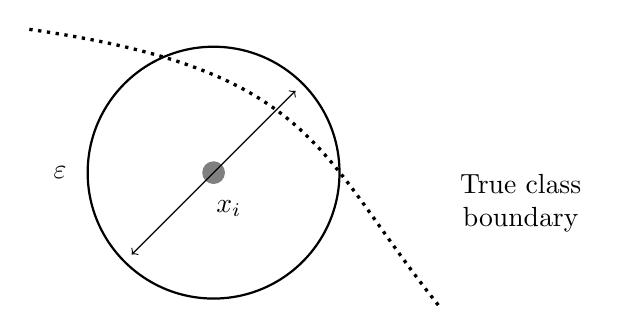
\begin{tikzpicture}[scale=1.3]
        \draw [very thick,dotted] (-2,1.2) .. controls (0.8, 0.8) and (0.8,0) .. (2,-1.5);
        \filldraw [gray] (-0.2,-0.2) circle (3pt);
        \draw [->] (-0.5,-0.5) -- (0.6,0.6);
        \draw [->] (-0.5,-0.5) -- (-1,-1);
        \draw [thick] (-0.2,-0.2) circle (35pt);
        
        \node at (-0.05,-0.55) {$x_i$};
        \node at (-1.7, -0.2) {$\varepsilon$};
        \node[align=center] at (2.8, -0.5) {True class \\ boundary};
    \end{tikzpicture}
    \label{fig:complexity}
\end{figure}

\begin{center}
\vspace{2em}
Example where a data point \(x_i\) lies close to the class decision boundary. In these
situations, too large \(\varepsilon\) values, may push the synthetically generated
point over true class boundaries.
\end{center}
\end{frame}

\begin{frame}[label={sec:org4e03420}]{Estimated boundaries can be deceiving}
\begin{columns}
\begin{column}{0.5\columnwidth}
\begin{figure}
    \centering
    \begin{tikzpicture}[scale=1.3]
	% nodes
	\draw (-1,0) circle (3pt);
	\filldraw [gray] (1,0) circle (3pt);

	%lines
	\draw (0, 1) -- (0,-1);
	\draw [dotted] (-0.9,1) -- (-0.9,-1);
	\draw [dotted] ( 0.9,1) -- ( 0.9,-1);
    \end{tikzpicture}
    \label{fig:density_a}
\end{figure}

\begin{center}
\vspace{2em}Sparse regions of the manifold may appear simple due to the lack of information.
\end{center}
\end{column}

\begin{column}{0.5\columnwidth}
\begin{figure}
    \centering
    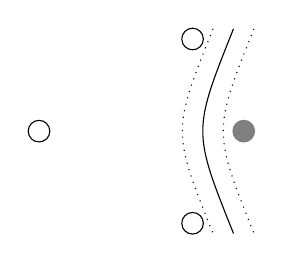
\begin{tikzpicture}[scale=1.3]
	% nodes
	\draw (-1,0) circle (3pt);
	\draw (0.5,0.9) circle (3pt);
	\draw (0.5,-0.9) circle (3pt);
	\filldraw [gray] (1,0) circle (3pt);

	%lines
	\draw (0.9, 1) .. controls (0.5,0) .. (0.9,-1);
	\draw [dotted] (1.1, 1) .. controls (0.7,0) .. (1.1,-1);
	\draw [dotted] (0.7, 1) .. controls (0.3,0) .. (0.7,-1);
    \end{tikzpicture}
    \label{fig:density_b}
\end{figure}


\begin{center}
\vspace{2em}More data points enable more precise estimation of the class boundary.
\end{center}
\end{column}
\end{columns}
\end{frame}

\begin{frame}[label={sec:org39e1d0d}]{Estimating Sparsity/Density}
\begin{equation}
    \varphi(x; \overline{x}) =  \frac{1}{\sqrt{1 + (\varepsilon r)^2}},\; \text{where}\; r = \parallel \overline{x} - x \parallel
    \label{eq:rbf}
\end{equation}

\vspace{2em}

We achieve a good measure of the density through the sum of the RBFs centred on all
data points \(X^c\) of class \(c\) (Eq.\textasciitilde{}\ref{eq:density}).

\vspace{2em}

\begin{equation}
    \rho_c(x) = \sum_{x_j \in X^c} \varphi(x; x_j)
    \label{eq:density}
\end{equation}
\end{frame}

\begin{frame}[label={sec:org1030207}]{Iterative expansion to create `adapted neighbourhoods'}
\begin{figure}
    \centering
    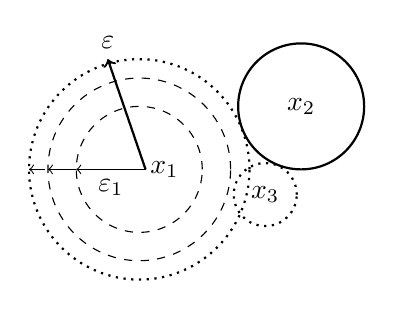
\begin{tikzpicture}[scale=.8]
        \draw (0.4,0) node {$x_1$};
        \draw[dashed] (0,0) circle (1.0cm);
        \draw[dashed] (0,0) circle (1.45cm);
        \draw[thick,dotted] (0,0) circle (1.75cm);
        
        \draw[->]        (0.1,0) -- (-1.0,0) node[below,midway] {$\varepsilon_1$};
        \draw[->] (-1.0,0) -- (-1.45,0) node[below,midway] {};
        \draw[->] (-1.5,0) -- (-1.75,0) node[below,midway] {};
        \draw[thick, ->] (0.1,0) -- (-0.5,1.75) node[anchor=south] {$\varepsilon$};
        
        \draw (2.57,1) node {$x_2$};
        \draw[thick] (2.57,1) circle (1.0cm);
        
        \draw (2,-0.4) node {$x_3$};
        \draw[thick,dotted] (2,-0.4) circle (0.5cm);
    \end{tikzpicture}
\label{fig:e_expansion}
\end{figure}

\begin{center}
\vspace{2em}Iterative \(\varepsilon\)-expansion process in a binary class scenario. The
two classes are distinguished by the dotted and solid circles.\vspace{1em}
\end{center}

\begin{equation*}
    \Delta\varepsilon_i^n=e^{-\rho_{c(i)}(x_i) \cdot n}
    \label{eq:step}
\end{equation*}
\end{frame}

\section{Results}
\label{sec:org95f06ef}

\begin{frame}[label={sec:orgf29c018},plain,c]{}
\begin{center}
\vspace{1em}\Huge Results
\end{center}
\end{frame}

\begin{frame}[label={sec:orgbb6578c}]{Aim of Experimentation}
We'd like to answer the following:
\begin{enumerate}
\item Does using adaptive neighbourhood provide any benefit? Why use it at all?
\item Can existing methods work for non-image based datasets, or do we need to design
new methods entirely?
\end{enumerate}
\end{frame}




\begin{frame}[label={sec:orge9d0460}]{Classification of Iris flowers -- problem statement}
\begin{columns}
\begin{column}{0.3\columnwidth}
\begin{center}
\includegraphics[width=1.0\textwidth]{images/Petal-sepal.jpg}
\end{center}
\end{column}

\begin{column}{0.7\columnwidth}
\begin{figure}
    \centering
    \includegraphics[width=\textwidth]{images/iris-eps.png}
    \label{fig:iris}
\end{figure}

(Jay Morgan and Adeline Paiement and Arno Pauly and Monika Seisenberger, 2021)
\end{column}
\end{columns}
\end{frame}

\begin{frame}[label={sec:org75a0b42}]{Attack and defence results for the Iris dataset classification task}
\begin{table}
\centering
\begin{adjustbox}{center}
\resizebox{\textwidth}{!}{\begin{tabular}[t]{cccccc}
\toprule
\multicolumn{2}{c}{ } & \multicolumn{4}{c}{Attack} \\
\cmidrule(l{3pt}r{3pt}){3-6}
Defence & None & FGSM & PGD & FGSM+AN & PGD+AN\\
\midrule
None & 0.9745 (0.0413) & \textcolor{red}{0.9278 (0.0618)} & 0.8572 (0.1036) & \textcolor{red}{0.7764 (0.0813)} & 0.8461 (0.0968)\\
FGSM & 0.9811 (0.0396) & 0.9408 (0.0757) & 0.8468 (0.1080) & 0.7873 (0.0785) & 0.8448 (0.0698)\\
PGD & 0.9867 (0.0400) & 0.9462 (0.0740) & 0.8680 (0.0740) & 0.8508 (0.0746) & 0.8759 (0.0823)\\
\midrule
Random+AN & 0.9936 (0.0193) & 0.9272 (0.0620) & 0.8274 (0.0918) & 0.7935 (0.0822) & 0.8454 (0.0864)\\
FGSM+AN & 0.9936 (0.0193) & \textcolor{red}{0.9406 (0.0745)} & 0.8420 (0.0987) & \textcolor{red}{0.8140 (0.1085)} & 0.8588 (0.1157)\\
PGD+AN & 0.9936 (0.0193) & 0.9472 (0.0642) & 0.9472 (0.0642) & 0.8679 (0.0899) & 0.8753 (0.0864)\\
\bottomrule
\end{tabular}}
\end{adjustbox}
\end{table}

\begin{center}
What we learn here then is that our adaptive neighbourhoods is able to strengthen the
form of adversarial attack and defence.
\end{center}
\end{frame}

\begin{frame}[label={sec:orge92ca2e}]{Adversarial examples in a Solar Burst Detection task -- problem statement}
\begin{figure}[t]
\centering
\resizebox{0.55\textwidth}{!}{% Created by tikzDevice version 0.12.3.1 on 2021-08-05 13:47:53
% !TEX encoding = UTF-8 Unicode
\begin{tikzpicture}[x=1pt,y=1pt]
\definecolor{fillColor}{RGB}{255,255,255}
\path[use as bounding box,fill=fillColor,fill opacity=0.00] (0,0) rectangle (433.62,542.02);
\begin{scope}
\path[clip] ( 15.84,406.52) rectangle (128.70,542.02);
\node[inner sep=0pt,outer sep=0pt,anchor=south west,rotate=  0.00] at ( 24.71, 406.52) {
	\pgfimage[width= 95.12pt,height=135.51pt,interpolate=true]{images/adversarial_example_ras1}};
\end{scope}
\begin{scope}
\path[clip] ( 15.84,406.52) rectangle (128.70,542.02);
\definecolor{drawColor}{RGB}{255,0,0}

\path[draw=drawColor,line width= 0.4pt,line join=round,line cap=round] ( 32.68,542.02) rectangle ( 47.56,454.34);
\end{scope}
\begin{scope}
\path[clip] (  0.00,  0.00) rectangle (433.62,542.02);
\definecolor{drawColor}{RGB}{0,0,0}

\node[text=drawColor,anchor=base west,inner sep=0pt, outer sep=0pt, scale=  1.30] at (139.79,469.80) {+};
\end{scope}
\begin{scope}
\path[clip] (160.38,406.52) rectangle (273.24,542.02);
\node[inner sep=0pt,outer sep=0pt,anchor=south west,rotate=  0.00] at (171.88, 406.52) {
	\pgfimage[width= 89.85pt,height=135.51pt,interpolate=true]{images/adversarial_example_ras2}};
\end{scope}
\begin{scope}
\path[clip] (  0.00,  0.00) rectangle (433.62,542.02);
\definecolor{drawColor}{RGB}{0,0,0}

\node[text=drawColor,anchor=base west,inner sep=0pt, outer sep=0pt, scale=  1.30] at (284.33,469.80) {=};
\end{scope}
\begin{scope}
\path[clip] (304.92,406.52) rectangle (417.78,542.02);
\node[inner sep=0pt,outer sep=0pt,anchor=south west,rotate=  0.00] at (313.79, 406.52) {
	\pgfimage[width= 95.12pt,height=135.51pt,interpolate=true]{images/adversarial_example_ras3}};
\end{scope}
\begin{scope}
\path[clip] (304.92,406.52) rectangle (417.78,542.02);
\definecolor{drawColor}{RGB}{0,0,255}

\path[draw=drawColor,line width= 0.4pt,line join=round,line cap=round] (320.17,540.96) rectangle (339.30,444.78);

\path[draw=drawColor,line width= 0.4pt,line join=round,line cap=round] (321.76,542.56) rectangle (331.86,449.56);
\end{scope}
\begin{scope}
\path[clip] ( 15.84,271.01) rectangle (128.70,406.52);
\node[inner sep=0pt,outer sep=0pt,anchor=south west,rotate=  0.00] at ( 24.71, 271.01) {
	\pgfimage[width= 95.12pt,height=135.51pt,interpolate=true]{images/adversarial_example_ras4}};
\end{scope}
\begin{scope}
\path[clip] ( 15.84,271.01) rectangle (128.70,406.52);
\definecolor{drawColor}{RGB}{255,0,0}

\path[draw=drawColor,line width= 0.4pt,line join=round,line cap=round] ( 32.68,406.52) rectangle ( 47.56,318.84);
\end{scope}
\begin{scope}
\path[clip] (  0.00,  0.00) rectangle (433.62,542.02);
\definecolor{drawColor}{RGB}{0,0,0}

\node[text=drawColor,anchor=base west,inner sep=0pt, outer sep=0pt, scale=  1.30] at (139.79,334.29) {+};
\end{scope}
\begin{scope}
\path[clip] (160.38,271.01) rectangle (273.24,406.52);
\node[inner sep=0pt,outer sep=0pt,anchor=south west,rotate=  0.00] at (169.25, 271.01) {
	\pgfimage[width= 95.12pt,height=135.51pt,interpolate=true]{images/adversarial_example_ras5}};
\end{scope}
\begin{scope}
\path[clip] (  0.00,  0.00) rectangle (433.62,542.02);
\definecolor{drawColor}{RGB}{0,0,0}

\node[text=drawColor,anchor=base west,inner sep=0pt, outer sep=0pt, scale=  1.30] at (284.33,334.29) {=};
\end{scope}
\begin{scope}
\path[clip] (304.92,271.01) rectangle (417.78,406.52);
\node[inner sep=0pt,outer sep=0pt,anchor=south west,rotate=  0.00] at (313.79, 271.01) {
	\pgfimage[width= 95.12pt,height=135.51pt,interpolate=true]{images/adversarial_example_ras6}};
\end{scope}
\begin{scope}
\path[clip] (304.92,271.01) rectangle (417.78,406.52);
\definecolor{drawColor}{RGB}{0,0,255}

\path[draw=drawColor,line width= 0.4pt,line join=round,line cap=round] (320.17,405.46) rectangle (339.30,308.74);

\path[draw=drawColor,line width= 0.4pt,line join=round,line cap=round] (321.76,407.05) rectangle (331.86,313.52);

\path[draw=drawColor,line width= 0.4pt,line join=round,line cap=round] (385.00,334.25) rectangle (392.44,326.81);

\path[draw=drawColor,line width= 0.4pt,line join=round,line cap=round] (393.50,325.75) rectangle (398.28,321.50);

\path[draw=drawColor,line width= 0.4pt,line join=round,line cap=round] (389.78,307.68) rectangle (391.91,302.36);

\path[draw=drawColor,line width= 0.4pt,line join=round,line cap=round] (322.82,404.39) rectangle (328.67,337.97);

\path[draw=drawColor,line width= 0.4pt,line join=round,line cap=round] (326.01,407.05) rectangle (337.17,332.12);

\path[draw=drawColor,line width= 0.4pt,line join=round,line cap=round] (348.86,343.81) rectangle (354.71,333.19);

\path[draw=drawColor,line width= 0.4pt,line join=round,line cap=round] (382.34,324.15) rectangle (387.12,312.46);

\path[draw=drawColor,line width= 0.4pt,line join=round,line cap=round] (355.24,341.16) rectangle (364.27,333.19);

\path[draw=drawColor,line width= 0.4pt,line join=round,line cap=round] (373.31,280.05) rectangle (382.87,271.54);

\path[draw=drawColor,line width= 0.4pt,line join=round,line cap=round] (385.53,332.65) rectangle (390.31,328.40);

\path[draw=drawColor,line width= 0.4pt,line join=round,line cap=round] (392.97,278.98) rectangle (400.94,271.54);

\path[draw=drawColor,line width= 0.4pt,line join=round,line cap=round] (368.52,294.39) rectangle (373.31,290.14);

\path[draw=drawColor,line width= 0.4pt,line join=round,line cap=round] (386.06,333.19) rectangle (394.56,324.68);

\path[draw=drawColor,line width= 0.4pt,line join=round,line cap=round] (386.59,277.92) rectangle (398.81,272.61);

\path[draw=drawColor,line width= 0.4pt,line join=round,line cap=round] (366.93,296.52) rectangle (373.84,289.61);

\path[draw=drawColor,line width= 0.4pt,line join=round,line cap=round] (391.91,326.28) rectangle (398.81,320.43);

\path[draw=drawColor,line width= 0.4pt,line join=round,line cap=round] (381.28,325.21) rectangle (389.25,308.74);

\path[draw=drawColor,line width= 0.4pt,line join=round,line cap=round] (386.06,281.11) rectangle (390.84,271.54);

\path[draw=drawColor,line width= 0.4pt,line join=round,line cap=round] (375.43,308.21) rectangle (393.50,299.71);

\path[draw=drawColor,line width= 0.4pt,line join=round,line cap=round] (388.19,308.74) rectangle (392.44,300.24);

\path[draw=drawColor,line width= 0.4pt,line join=round,line cap=round] (395.09,285.89) rectangle (399.34,281.64);

\path[draw=drawColor,line width= 0.4pt,line join=round,line cap=round] (384.47,279.51) rectangle (402.00,271.54);

\path[draw=drawColor,line width= 0.4pt,line join=round,line cap=round] (390.84,290.14) rectangle (399.88,281.64);

\path[draw=drawColor,line width= 0.4pt,line join=round,line cap=round] (392.44,331.59) rectangle (397.75,321.50);

\path[draw=drawColor,line width= 0.4pt,line join=round,line cap=round] (393.50,286.95) rectangle (400.94,280.58);

\path[draw=drawColor,line width= 0.4pt,line join=round,line cap=round] (353.11,297.58) rectangle (362.15,293.33);

\path[draw=drawColor,line width= 0.4pt,line join=round,line cap=round] (377.56,308.74) rectangle (386.59,300.77);

\path[draw=drawColor,line width= 0.4pt,line join=round,line cap=round] (377.56,308.74) rectangle (387.65,304.49);

\path[draw=drawColor,line width= 0.4pt,line join=round,line cap=round] (384.47,333.72) rectangle (389.25,328.93);

\path[draw=drawColor,line width= 0.4pt,line join=round,line cap=round] (363.74,298.11) rectangle (371.71,290.67);

\path[draw=drawColor,line width= 0.4pt,line join=round,line cap=round] (394.03,318.84) rectangle (398.28,309.80);

\path[draw=drawColor,line width= 0.4pt,line join=round,line cap=round] (355.24,297.05) rectangle (361.08,294.39);

\path[draw=drawColor,line width= 0.4pt,line join=round,line cap=round] (385.00,335.31) rectangle (394.03,320.43);

\path[draw=drawColor,line width= 0.4pt,line join=round,line cap=round] (367.46,294.93) rectangle (372.24,290.67);

\path[draw=drawColor,line width= 0.4pt,line join=round,line cap=round] (390.31,291.21) rectangle (399.88,285.89);

\path[draw=drawColor,line width= 0.4pt,line join=round,line cap=round] (348.33,341.16) rectangle (365.34,332.65);

\path[draw=drawColor,line width= 0.4pt,line join=round,line cap=round] (387.12,325.75) rectangle (398.81,320.96);

\path[draw=drawColor,line width= 0.4pt,line join=round,line cap=round] (392.97,285.36) rectangle (397.22,281.11);

\path[draw=drawColor,line width= 0.4pt,line join=round,line cap=round] (381.81,324.15) rectangle (390.84,315.65);

\path[draw=drawColor,line width= 0.4pt,line join=round,line cap=round] (385.00,332.65) rectangle (403.60,324.68);

\path[draw=drawColor,line width= 0.4pt,line join=round,line cap=round] (384.47,333.19) rectangle (389.78,323.62);

\path[draw=drawColor,line width= 0.4pt,line join=round,line cap=round] (380.21,324.68) rectangle (387.65,316.71);

\path[draw=drawColor,line width= 0.4pt,line join=round,line cap=round] (388.72,307.68) rectangle (407.85,300.24);

\path[draw=drawColor,line width= 0.4pt,line join=round,line cap=round] (362.15,294.93) rectangle (372.78,290.14);

\path[draw=drawColor,line width= 0.4pt,line join=round,line cap=round] (397.22,306.08) rectangle (407.32,301.30);

\path[draw=drawColor,line width= 0.4pt,line join=round,line cap=round] (328.14,407.05) rectangle (349.92,289.08);

\path[draw=drawColor,line width= 0.4pt,line join=round,line cap=round] (380.75,324.15) rectangle (385.53,312.99);

\path[draw=drawColor,line width= 0.4pt,line join=round,line cap=round] (386.06,280.58) rectangle (395.09,272.08);

\path[draw=drawColor,line width= 0.4pt,line join=round,line cap=round] (390.84,332.65) rectangle (399.34,324.68);

\path[draw=drawColor,line width= 0.4pt,line join=round,line cap=round] (398.81,333.19) rectangle (405.72,325.75);

\path[draw=drawColor,line width= 0.4pt,line join=round,line cap=round] (346.74,343.81) rectangle (355.24,327.34);

\path[draw=drawColor,line width= 0.4pt,line join=round,line cap=round] (365.87,294.39) rectangle (370.12,290.67);

\path[draw=drawColor,line width= 0.4pt,line join=round,line cap=round] (346.74,344.35) rectangle (352.58,334.25);

\path[draw=drawColor,line width= 0.4pt,line join=round,line cap=round] (388.72,293.86) rectangle (397.75,278.45);

\path[draw=drawColor,line width= 0.4pt,line join=round,line cap=round] (394.03,317.78) rectangle (396.69,311.93);

\path[draw=drawColor,line width= 0.4pt,line join=round,line cap=round] (367.99,294.39) rectangle (372.78,291.74);

\path[draw=drawColor,line width= 0.4pt,line join=round,line cap=round] (383.93,322.56) rectangle (389.25,310.87);

\path[draw=drawColor,line width= 0.4pt,line join=round,line cap=round] (389.25,285.89) rectangle (399.34,280.58);

\path[draw=drawColor,line width= 0.4pt,line join=round,line cap=round] (384.47,281.11) rectangle (389.25,271.54);

\path[draw=drawColor,line width= 0.4pt,line join=round,line cap=round] (353.64,298.11) rectangle (374.37,290.14);

\path[draw=drawColor,line width= 0.4pt,line join=round,line cap=round] (385.00,332.65) rectangle (401.47,317.78);

\path[draw=drawColor,line width= 0.4pt,line join=round,line cap=round] (348.86,298.65) rectangle (361.08,293.86);

\path[draw=drawColor,line width= 0.4pt,line join=round,line cap=round] (356.30,322.56) rectangle (365.34,314.06);

\path[draw=drawColor,line width= 0.4pt,line join=round,line cap=round] (386.06,281.64) rectangle (390.31,276.86);

\path[draw=drawColor,line width= 0.4pt,line join=round,line cap=round] (397.22,298.11) rectangle (400.94,294.39);

\path[draw=drawColor,line width= 0.4pt,line join=round,line cap=round] (382.34,334.25) rectangle (399.34,326.28);

\path[draw=drawColor,line width= 0.4pt,line join=round,line cap=round] (381.28,326.28) rectangle (397.75,311.40);

\path[draw=drawColor,line width= 0.4pt,line join=round,line cap=round] (398.28,298.11) rectangle (399.88,294.93);

\path[draw=drawColor,line width= 0.4pt,line join=round,line cap=round] (388.19,332.65) rectangle (399.88,328.40);

\path[draw=drawColor,line width= 0.4pt,line join=round,line cap=round] (402.53,305.02) rectangle (406.78,300.77);

\path[draw=drawColor,line width= 0.4pt,line join=round,line cap=round] (387.12,277.92) rectangle (389.25,272.08);

\path[draw=drawColor,line width= 0.4pt,line join=round,line cap=round] (392.44,318.84) rectangle (396.69,310.34);

\path[draw=drawColor,line width= 0.4pt,line join=round,line cap=round] (381.28,325.21) rectangle (400.94,317.24);

\path[draw=drawColor,line width= 0.4pt,line join=round,line cap=round] (390.84,332.12) rectangle (402.00,327.34);

\path[draw=drawColor,line width= 0.4pt,line join=round,line cap=round] (394.56,304.49) rectangle (406.78,299.71);

\path[draw=drawColor,line width= 0.4pt,line join=round,line cap=round] (367.99,320.43) rectangle (372.78,310.34);

\path[draw=drawColor,line width= 0.4pt,line join=round,line cap=round] (392.44,306.08) rectangle (404.13,301.83);

\path[draw=drawColor,line width= 0.4pt,line join=round,line cap=round] (379.68,328.40) rectangle (387.65,312.46);

\path[draw=drawColor,line width= 0.4pt,line join=round,line cap=round] (355.77,312.46) rectangle (368.52,308.74);

\path[draw=drawColor,line width= 0.4pt,line join=round,line cap=round] (364.80,295.46) rectangle (369.59,291.21);

\path[draw=drawColor,line width= 0.4pt,line join=round,line cap=round] (349.92,321.50) rectangle (367.46,312.99);

\path[draw=drawColor,line width= 0.4pt,line join=round,line cap=round] (351.52,315.12) rectangle (370.65,307.68);

\path[draw=drawColor,line width= 0.4pt,line join=round,line cap=round] (385.00,327.34) rectangle (397.75,322.56);

\path[draw=drawColor,line width= 0.4pt,line join=round,line cap=round] (345.14,303.43) rectangle (355.24,299.18);

\path[draw=drawColor,line width= 0.4pt,line join=round,line cap=round] (350.99,340.63) rectangle (363.21,335.84);

\path[draw=drawColor,line width= 0.4pt,line join=round,line cap=round] (382.34,323.09) rectangle (395.63,317.78);

\path[draw=drawColor,line width= 0.4pt,line join=round,line cap=round] (351.52,331.59) rectangle (353.11,328.40);

\path[draw=drawColor,line width= 0.4pt,line join=round,line cap=round] (383.93,302.36) rectangle (385.53,299.18);

\path[draw=drawColor,line width= 0.4pt,line join=round,line cap=round] (349.92,323.09) rectangle (354.18,313.52);

\path[draw=drawColor,line width= 0.4pt,line join=round,line cap=round] (386.06,327.34) rectangle (406.25,319.37);

\path[draw=drawColor,line width= 0.4pt,line join=round,line cap=round] (405.19,332.65) rectangle (407.85,326.81);

\path[draw=drawColor,line width= 0.4pt,line join=round,line cap=round] (382.87,324.68) rectangle (395.63,319.37);

\path[draw=drawColor,line width= 0.4pt,line join=round,line cap=round] (396.69,298.65) rectangle (398.28,295.46);

\path[draw=drawColor,line width= 0.4pt,line join=round,line cap=round] (351.52,332.12) rectangle (353.11,329.47);

\path[draw=drawColor,line width= 0.4pt,line join=round,line cap=round] (380.75,331.59) rectangle (399.34,322.56);

\path[draw=drawColor,line width= 0.4pt,line join=round,line cap=round] (364.27,293.33) rectangle (365.87,291.21);

\path[draw=drawColor,line width= 0.4pt,line join=round,line cap=round] (352.58,323.09) rectangle (369.06,308.21);

\path[draw=drawColor,line width= 0.4pt,line join=round,line cap=round] (322.82,293.33) rectangle (356.83,272.61);
\end{scope}
\begin{scope}
\path[clip] ( 15.84,135.51) rectangle (128.70,271.01);
\node[inner sep=0pt,outer sep=0pt,anchor=south west,rotate=  0.00] at ( 24.71, 135.51) {
	\pgfimage[width= 95.12pt,height=135.51pt,interpolate=true]{images/adversarial_example_ras7}};
\end{scope}
\begin{scope}
\path[clip] ( 15.84,135.51) rectangle (128.70,271.01);
\definecolor{drawColor}{RGB}{255,0,0}

\path[draw=drawColor,line width= 0.4pt,line join=round,line cap=round] ( 32.68,271.01) rectangle ( 47.56,183.33);
\end{scope}
\begin{scope}
\path[clip] (  0.00,  0.00) rectangle (433.62,542.02);
\definecolor{drawColor}{RGB}{0,0,0}

\node[text=drawColor,anchor=base west,inner sep=0pt, outer sep=0pt, scale=  1.30] at (139.79,198.78) {+};
\end{scope}
\begin{scope}
\path[clip] (160.38,135.51) rectangle (273.24,271.01);
\node[inner sep=0pt,outer sep=0pt,anchor=south west,rotate=  0.00] at (169.25, 135.51) {
	\pgfimage[width= 95.12pt,height=135.51pt,interpolate=true]{images/adversarial_example_ras8}};
\end{scope}
\begin{scope}
\path[clip] (  0.00,  0.00) rectangle (433.62,542.02);
\definecolor{drawColor}{RGB}{0,0,0}

\node[text=drawColor,anchor=base west,inner sep=0pt, outer sep=0pt, scale=  1.30] at (284.33,198.78) {=};
\end{scope}
\begin{scope}
\path[clip] (304.92,135.51) rectangle (417.78,271.01);
\node[inner sep=0pt,outer sep=0pt,anchor=south west,rotate=  0.00] at (313.79, 135.51) {
	\pgfimage[width= 95.12pt,height=135.51pt,interpolate=true]{images/adversarial_example_ras9}};
\end{scope}
\begin{scope}
\path[clip] (304.92,135.51) rectangle (417.78,271.01);
\definecolor{drawColor}{RGB}{0,0,255}

\path[draw=drawColor,line width= 0.4pt,line join=round,line cap=round] (320.17,269.95) rectangle (339.30,173.24);

\path[draw=drawColor,line width= 0.4pt,line join=round,line cap=round] (321.76,271.54) rectangle (331.86,178.02);

\path[draw=drawColor,line width= 0.4pt,line join=round,line cap=round] (322.82,268.89) rectangle (328.67,202.46);

\path[draw=drawColor,line width= 0.4pt,line join=round,line cap=round] (326.01,271.54) rectangle (337.17,196.62);

\path[draw=drawColor,line width= 0.4pt,line join=round,line cap=round] (320.17,271.54) rectangle (361.62,186.52);

\path[draw=drawColor,line width= 0.4pt,line join=round,line cap=round] (373.84,240.72) rectangle (375.43,235.41);

\path[draw=drawColor,line width= 0.4pt,line join=round,line cap=round] (328.14,271.54) rectangle (349.92,152.51);

\path[draw=drawColor,line width= 0.4pt,line join=round,line cap=round] (372.78,243.38) rectangle (375.96,233.81);

\path[draw=drawColor,line width= 0.4pt,line join=round,line cap=round] (340.89,148.26) rectangle (364.27,138.69);

\path[draw=drawColor,line width= 0.4pt,line join=round,line cap=round] (322.82,157.82) rectangle (356.83,137.10);

\path[draw=drawColor,line width= 0.4pt,line join=round,line cap=round] (333.98,156.76) rectangle (352.58,141.35);

\path[draw=drawColor,line width= 0.4pt,line join=round,line cap=round] (322.82,243.38) rectangle (328.14,191.30);

\path[draw=drawColor,line width= 0.4pt,line join=round,line cap=round] (335.05,171.11) rectangle (356.83,136.57);

\path[draw=drawColor,line width= 0.4pt,line join=round,line cap=round] (333.45,163.67) rectangle (370.12,135.51);
\end{scope}
\begin{scope}
\path[clip] ( 15.84,  0.00) rectangle (128.70,135.51);
\node[inner sep=0pt,outer sep=0pt,anchor=south west,rotate=  0.00] at ( 24.71,   0.00) {
	\pgfimage[width= 95.12pt,height=135.51pt,interpolate=true]{images/adversarial_example_ras10}};
\end{scope}
\begin{scope}
\path[clip] ( 15.84,  0.00) rectangle (128.70,135.51);
\definecolor{drawColor}{RGB}{255,0,0}

\path[draw=drawColor,line width= 0.4pt,line join=round,line cap=round] ( 32.68,135.51) rectangle ( 47.56, 47.83);
\end{scope}
\begin{scope}
\path[clip] (  0.00,  0.00) rectangle (433.62,542.02);
\definecolor{drawColor}{RGB}{0,0,0}

\node[text=drawColor,anchor=base west,inner sep=0pt, outer sep=0pt, scale=  1.30] at (139.79, 63.28) {+};
\end{scope}
\begin{scope}
\path[clip] (160.38,  0.00) rectangle (273.24,135.51);
\node[inner sep=0pt,outer sep=0pt,anchor=south west,rotate=  0.00] at (169.25,   0.00) {
	\pgfimage[width= 95.12pt,height=135.51pt,interpolate=true]{images/adversarial_example_ras11}};
\end{scope}
\begin{scope}
\path[clip] (  0.00,  0.00) rectangle (433.62,542.02);
\definecolor{drawColor}{RGB}{0,0,0}

\node[text=drawColor,anchor=base west,inner sep=0pt, outer sep=0pt, scale=  1.30] at (284.33, 63.28) {=};
\end{scope}
\begin{scope}
\path[clip] (304.92,  0.00) rectangle (417.78,135.51);
\node[inner sep=0pt,outer sep=0pt,anchor=south west,rotate=  0.00] at (313.79,   0.00) {
	\pgfimage[width= 95.12pt,height=135.51pt,interpolate=true]{images/adversarial_example_ras12}};
\end{scope}
\begin{scope}
\path[clip] (304.92,  0.00) rectangle (417.78,135.51);
\definecolor{drawColor}{RGB}{0,0,255}

\path[draw=drawColor,line width= 0.4pt,line join=round,line cap=round] (320.17,134.44) rectangle (339.30, 38.26);

\path[draw=drawColor,line width= 0.4pt,line join=round,line cap=round] (321.76,136.04) rectangle (331.86, 42.51);

\path[draw=drawColor,line width= 0.4pt,line join=round,line cap=round] (320.70,129.13) rectangle (337.17, 76.52);

\path[draw=drawColor,line width= 0.4pt,line join=round,line cap=round] (322.82,133.38) rectangle (328.67, 66.42);

\path[draw=drawColor,line width= 0.4pt,line join=round,line cap=round] (322.82, 24.98) rectangle (357.90,  3.19);

\path[draw=drawColor,line width= 0.4pt,line join=round,line cap=round] (320.17,136.04) rectangle (361.08, 50.48);

\path[draw=drawColor,line width= 0.4pt,line join=round,line cap=round] (327.07,133.38) rectangle (337.17, 45.17);

\path[draw=drawColor,line width= 0.4pt,line join=round,line cap=round] (328.14,136.04) rectangle (349.39, 15.41);

\path[draw=drawColor,line width= 0.4pt,line join=round,line cap=round] (322.82,108.41) rectangle (328.14, 55.80);
\end{scope}
\end{tikzpicture}
}
\label{fig:adv_example}
\end{figure}
(Jay Morgan, 2022)
\end{frame}

\begin{frame}[label={sec:org23d4987}]{Attack and defence results for the solar bursts task}
\begin{table}
\centering
\begin{adjustbox}{center}
\resizebox{\textwidth}{!}{\begin{tabular}[t]{rccccccc}
\toprule
\multicolumn{2}{c}{ } & \multicolumn{6}{c}{Attack} \\
\cmidrule(l{3pt}r{3pt}){3-8}
Defence & None & FGSM & FGSM+AN & PGD & PGD+AN & DAG & DAG+AN\\
\midrule
None & 0.568 & \textcolor{red}{0.539} & \textcolor{red}{0.486} & 0.198 & 0.105 & 0.399 & 0.251\\
FGSM & 0.463 & \textcolor{red}{0.458} & 0.178 & 0.013 & 0.012 & 0.055 & 0.028\\
FGSM+AN & 0.480 & \textcolor{red}{0.465} & 0.462 & 0.007 & 0.007 & 0.043 & 0.023\\
PGD & 0.421 & 0.425 & 0.379 & 0.391 & 0.359 & 0.378 & 0.259\\
PGD+AN & 0.364 & 0.359 & 0.330 & 0.339 & 0.324 & 0.330 & 0.212\\
\bottomrule
\end{tabular}}
\end{adjustbox}
\end{table}

\begin{center}
Like our previous task, we see that, through the combination with adaptive
neighbourhoods, the attack is more successful. And likewise the defence is more
powerful.
\end{center}
\end{frame}

\section{Conclusion}
\label{sec:org915a0e0}

\begin{frame}[label={sec:org3a26648}]{Summary of Results}
We'd like to answer the following:
\begin{enumerate}
\item Does using adaptive neighbourhood provide any benefit? Why use it at all? -
\alert{Adaptive neighbourhoods is an effective method that compliments existing adversarial generation methods such as FGSM \& PGD.}
\item Can existing methods work for non-image based datasets, or do we need to design
new methods entirely? - \alert{Through the use of adaptive neighbourhoods, one can
meaningfully define searchable regions for datasets other than image-based data
where adversarial examples can be visually inspected.}
\end{enumerate}
\end{frame}

\begin{frame}[label={sec:org093242c}]{Source code}
\begin{center}
\includegraphics[width=0.8\textwidth]{images/github-repo.png}
\end{center}

\begin{center}
\url{https://github.com/jaypmorgan/adaptive-neighbourhoods}
\url{https://gibtlab.com/jaymorgan/adaptive-neighbourhoods}
\url{https://git.sr.ht/~jaymorgan/adaptive-neighbourhoods}
\end{center}
\end{frame}

\begin{frame}[label={sec:orgbcbd8ce}]{Link to the Slides}
\begin{center}
\includegraphics[width=1.0\textwidth]{images/presentations.png}
\end{center}

\begin{center}
\url{https://github.com/jaypmorgan/presentations}
\end{center}
\end{frame}

\begin{frame}[label={sec:org24fee9d},plain,c]{}
\begin{center}
\vspace{1em}\Huge Thank you!
\end{center}
\end{frame}

\begin{frame}[label={sec:org1daeff4}]{References}
\noindent
Goodfellow, Ian J and Shlens, Jonathon and Szegedy, Christian (2014). \emph{Explaining and harnessing adversarial examples}, arXiv preprint arXiv:1412.6572.

\noindent
Huang, Xiaowei and Kwiatkowska, Marta and Wang, Sen and Wu, Min (2017). \emph{Safety verification of deep neural networks}.

\noindent
Jay Morgan (2022). \emph{Strategies to use Prior Knowledge to Improve the Performance of Deep Learning}.

\noindent
Jay Morgan and Adeline Paiement and Arno Pauly and Monika Seisenberger (2021). \emph{Adaptive Neighbourhoods for the Discovery of Adversarial Examples}, CoRR.

\noindent
Madry, Aleksander and Makelov, Aleksandar and Schmidt, Ludwig and Tsipras, Dimitris and Vladu, Adrian (2017). \emph{Towards deep learning models resistant to adversarial attacks}, arXiv preprint arXiv:1706.06083.

\noindent
Potdar, Kedar and Pai, Chinmay and Akolkar, Sukrut (2018). \emph{A Convolutional Neural Network based Live Object Recognition System as Blind Aid}.
\end{frame}
\end{document}
